\documentclass{beamer}
%
% Choose how your presentation looks.
%
% For more themes, color themes and font themes, see:
% http://deic.uab.es/~iblanes/beamer_gallery/index_by_theme.html
%
\mode<presentation>
{
  \usetheme{default}      % or try Darmstadt, Madrid, Warsaw, ...
  \usecolortheme{crane} % or try albatross, beaver, crane, ...
  \usefonttheme{structurebold}  % or try serif, structurebold, ...
  \setbeamertemplate{navigation symbols}{}
  \setbeamertemplate{caption}[numbered]
} 

\usepackage[english]{babel}
\usepackage[utf8x]{inputenc}

\title[ML]{Machine Learning}
\author{Pawel Wocjan}
\institute{University of Central Florida}
\date{Fall 2020}

\begin{document}

\begin{frame}
  \titlepage
\end{frame}

\begin{frame}{An Iterative Approach}

\begin{itemize}
\item We now examine how a machine learning model reduces loss iteratively.

\medskip    
\item Iterative learning is reminiscent of the ``Hot and Cold'' kid's game for finding a hidden object. 

\medskip    
\item The ``hidden object'' is the best possible model. 

\medskip    
\item We start with a wild guess \emph{the value of $w_1$ is $0$} and wait for the system to tell us what the loss is. 
    
\medskip
Then, we try another guess \emph{The value of $w_1$ is $0.5$} and see what the loss is etc.
    
\medskip
\item If we adapt the weights cleverly, we will usually be decreasing the loss. 

\medskip
\item The real challenge is to find the best possible model as efficiently as possible.
\end{itemize}

\end{frame}

%%%

\begin{frame}{An Iterative Approach}
\begin{itemize}
    \item The figure below depicts the iterative trial-and-error process that machine learning algorithms use to train a model:
\end{itemize}

\bigskip
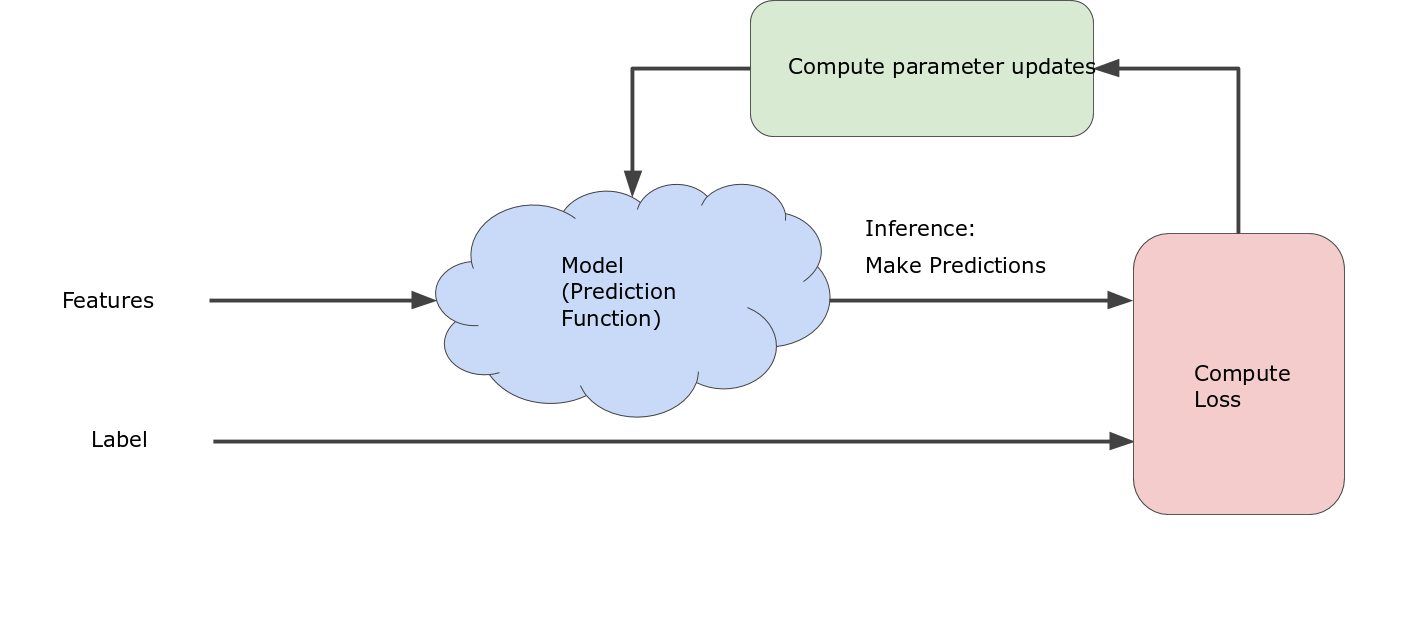
\includegraphics[width=\textwidth]{images/GradientDescentDiagram.png}
\end{frame}

\begin{frame}{An Iterative Approach}
\begin{itemize}    
\item Iterative strategies are prevalent in machine learning, primarily because they scale so well to large data sets.

\medskip
\item The model takes features $x_1,\ldots,x_n$ as input and returns one prediction $\hat{y}$ as output. 
    
\medskip
\item To simplify the discussion, consider the simplest linear regression model that takes only one feature as input:

$$ \hat{y} = b + w_1 x_1 $$

\end{itemize}
\end{frame}

%%%

\begin{frame}{An Iterative Approach}
\begin{itemize}
\item What initial values should we set for $b$ and $w_1$? 

\medskip 
\item For linear regression problems, it turns out that the starting values aren't important. 


\medskip
\item We could pick random values, but we'll just take the following trivial values instead:
    
$$ b = 0\,, \quad w_1 = 0 $$

\end{itemize}
\end{frame}

%%%

\begin{frame}{An Iterative Approach}
\begin{itemize}
\item Let us examine what happens inside the ``Compute parameter updates'' part of the diagram. 

\medskip
\item It is here that the ML system examines the value of the loss function and generates new values for $b$ and $w_1$. 

\medskip
\item For now, just assume that this mysterious box devises new values and then the ML system re-evaluates all those features against all those labels, yielding a new value for the loss function, which yields new parameter values. 

\medskip
\item The learning continues iterating until the ML system discovers the model parameters with the lowest possible loss. 

\medskip
\item Usually, we iterate until the loss stops changing or at least changes extremely slowly. When that happens, we say that the model has {\bf converged}.
\end{itemize}
\end{frame}

%%%

\begin{frame}{Key Point}
\begin{itemize}
    \item A ML model is trained by starting with an initial guess for the weights and the bias and iteratively adjusting those guesses until finding the weights and the bias with the lowest possible (or sufficiently low) loss are found.
\end{itemize}
\end{frame}

\begin{frame}{Key Terms}
\begin{itemize}
    \item convergence
    \item loss
    \item training
\end{itemize}
\end{frame}

\end{document}